\documentclass[a4paper]{tp}
\usepackage{listings}
\titre{TP20 : Pendule simple}
\begin{document}
%\small

\section{Objectif du TP}
L'objectif de ce TP est de faire l'acquisition de l'accélération d'un pendule simple à l'aide de l'accéléromètre d'un téléphone portable et d'analyser les données obtenues.

\vspace{1em}
\textit{Ne pas oublier qu'une mesure physique doit toujours être associée à une incertitude expérimentale. Penser à lire la notice des appareils pour connaître l'incertitude liée aux valeurs qu'ils fournissent.}

\section{Aspects théoriques}

\begin{center}
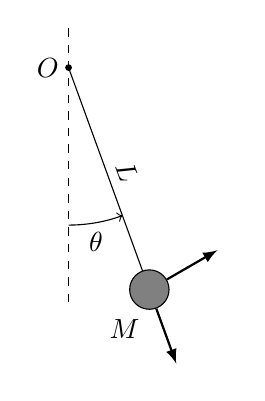
\begin{tikzpicture}
\draw[dashed] (0,0.5) -- (0,-3);
\draw[fill=black] (0,0) circle(1pt) coordinate (O) node[left]{$O$};
\draw (O) -- ++(-70:3) node[midway,above,sloped]{$L$} node[circle,fill=gray,draw=black,minimum height=0.5cm](M){};
\draw (M.south) node[below left]{$M$};
\draw[thick, -latex] (M) -- ++(-70:1) node[right]{$\ver$}; 
\draw[thick, -latex] (M) -- ++(30:1) node[right]{$\vet$}; 
\draw[->] (0,-2) arc (-90:-70:2) node[midway,below] {$\theta$};
\end{tikzpicture}

\end{center}

L'application des lois du mouvement (lois du Newton) au pendule simple permet d'obtenir l'équation différentielle du mouvement suivante :
\begin{equation*}
\ddot{\theta} + \frac{g}{l} \sin\theta = 0
\end{equation*}
qui nécessite une résolution numérique. Cependant, lorsque $\theta\ll 1$ on peut faire l'approximation $\sin\theta\simeq\theta$ et on obtient l'équation d'un oscillateur harmonique 
\begin{equation*}
\ddot{\theta} + \omega_0^2\theta = 0
\end{equation*}

Avec $\omega_0^2=\frac{g}{l}$. La période $T_0=\frac{2\pi}{\omega_0}=2\pi\sqrt{\frac{l}{g}}$ des oscillations ne dépend alors pas de leur amplitude. Pour des oscillations d'amplitude supérieures (mais ne dépassant pas \SI{60}{\degree}, on peut montrer que la période est donnée par la formule de Borda :

\begin{equation}
 T\simeq T_0 \left(1+\frac{\theta_0^2}{16}\right)
 \label{eq:borda}
\end{equation}

où $\theta_0$ est l'amplitude angulaire des oscillations.

Lorsqu'on ajoute une force de frottement fluide proportionnelle à la vitesse du pendule, on obtient l'équation d'un oscillateur harmonique amorti :
\begin{equation*}
\ddot{\theta} + \frac{\omega_0}{Q}\dot{\omega} + \omega_0^2 \sin\theta = 0
\end{equation*}
qui, lorsque $Q$ est élevé (c'est en général le cas) possède une solution pseudo-périodique :
\begin{equation*}
\theta(t) = \theta_0e^{-t/\tau}\sin(\omega t + \varphi)
\end{equation*}
où $\tau=2Q/\omega_0$ est le temps caractéristique d'amortissement du pendule et $\varphi$ la phase à l'origine.

Dans ce TP, nous allons mesurer l'accélération à l'aide d'un smartphone placé à la place de la masse. On s'arrangera pour qu'un des axes de l'accéléromètre du smartphone pointe dans la direction $\ver$ et l'autre dans la direction $\vet$.   

Le mouvement du pendule étant circulaire, l'accélération suivant $\ver$ est :
\begin{equation}
  a_r = -L \dot{\theta}^2 
\end{equation}

On peu alors montrer que $a_r(t)$ est de la forme
\begin{equation}
  a_r(t) = L \dot{\theta}^2 = A e^{-\frac{2t}{\tau}}\sin(\omega_0t + \varphi')^2
\end{equation}

On peut aussi montrer que sur une période d'oscillation, l'accélération normale est maximale lorsque le point $M$ se trouve à la verticale du point $O$ et vaut
\begin{equation}
  a_{rm} = 2g(1-\cos(\theta_0))
\end{equation}

\section{Manipulations}%
\label{sec:manipulations}

Pour faire les mesures d'accélération, vous utiliserez votre smartphone avec l'application \texttt{phyphox} que vous pouvez installer à partir de f-droid, Google Play ou App Store. 

Dans l'application \texttt{phyphox}, choisir le capteur "Accélération (sans g)". Vous pouvez alors lancer l'acquisition avec l'icone \includegraphics[]{images/phyphox_play.png}. À la fin de l'expérience, arrêtez l'acquisition en appuyant sur \includegraphics[]{images/phyphox_pause.png}. 

On cherche ici à mesurer l'accélération d'un pendule simple en fonction du temps. Il faudra donc fabriquer un pendule simple dont la masse oscillante est un smartphone contenant un accéléromètre (tous les smartphones contiennent des accéléromètres !). Les axes de l'accéléromètre du téléphone sont alignés avec les axes du téléphone. On s'arrangera pour que l'un de ces axes soit dans la direction du fil du pendule.

Écarter le pendule de sa position d'équilibre avec un angle assez grand, et faire l'acquisition des oscillations jusqu'à ce qu'elles soient très faibles.

Une fois que l'acquisition que vous vouliez faire est terminée, il faut exporter les données vers un fichier pour pouvoir les traiter avec python. Pour cela, appuyer sur \includegraphics[]{images/phyphox_opt.png}, puis "Exporter les mesures" et choisir "CSV (Tabulator, decimal point). Enregistrer le fichier sur le téléphone et le transférer sur l'ordinateur, vous devriez avoir un fichier compressé au format \texttt{zip} duquel il faudra extraire le fichier \texttt{csv} (probablement appelé \texttt{Raw Data.csv"}.

Une fois que vous avez le fichier \texttt{.csv} enregistré sur l'ordinateur, vous pouvez l'importer dans un tableau \texttt{numpy} pour commencer le traitement des données. 

\section{Traitement des données}%
\label{sec:traitement_des_donnees}

Supposons que le fichier contenant les données d'accélération que vous avez enregistrées s'appelle \texttt{data.csv} et que votre script python se trouve dans le même dossier que ce fichier. Pour importer les données dans un tableau numpy, vous pouvez faire :

\begin{minted}{python}
import numpy as np
data = np.loadtxt('data.csv', skiprows=1)
\end{minted}

Il faudra ensuite déterminer à quel axe de l'accéléromètre correspond l'accélération normale du pendule. Pour cela on pourra tracer les accélérations des trois axes en fonction du temps et cherche celle qui oscille le plus. On peut faire :

\begin{minted}{python}
import matplotlib.pyplot as plt
plt.plot(data[:,0], data[:,1])  # Axe x
plt.plot(data[:,0], data[:,2])  # Axe y
plt.plot(data[:,0], data[:,3])  # Axe z
\end{minted}

Une fois l'axe de l'accélération normale déterminé, on pourra garder les données correspondantes dans les tableaux \texttt{t} et \texttt{ar} avec

\begin{minted}{python}
t, ar = data[:,0], data[:,2]
\end{minted}

Vous devriez obtenir quelque-chose qui ressemble à ça :
\begin{center}
  \includegraphics[width=12cm]{images/tp20_raw.pdf}
\end{center}

Filtre ensuite ces deux tableaux pour ne conserver que les données correspondant aux oscillations du pendule en faisant:

\begin{minted}{python}
tmin = 2.2  # début des oscillations libres en s
tmax = 74   # fin des oscillations libres en s
tf = t[(t>tmin) & (t<tmax)] 
arf = ar[(t>tmin) & (t<tmax)] 

# On applique une moyenne glissante sur les données pour les lisser (filtre passe-bas)
n = 20    # nombre de points de la moyenne glissante
arf = np.convolve(arf,np.ones(n)/n,'same')
\end{minted}

Pour obtenir ceci : 
\begin{center}
  \includegraphics[width=12cm]{images/tp20_filtre.pdf}
\end{center}

On peut maintenant écrire un programme qui détecte les maxima d'accélération et qui détermine l'évolution de la période au cours du temps

\begin{minted}{python}
tdiff = tf[:-1]
diff = arf[1:]-arf[:-1] # liste des différences entre deux points successifs
diff = np.convolve(diff, np.ones(n)/n, 'same') # moyenne glissant pour lisser la courbe
i=0
lt = []  # liste des temps
la = []  # liste des accélérations
while i<len(diff)-1:
    if diff[i+1]<0 and diff[i]>0: # On cherche un changement de signe
        lt.append(tf[i])
        la.append(arf[i])
        i+=50          # On passe un certain nombre de points pour s'écarter du max
    i+=1
lt = np.array(lt[1:][::2]) # On oublie le premier et on garde un maximum sur 2
la = np.array(la[1:][::2])  
\end{minted}

On devrait pouvoir détecter les maxima et les accélérations correspondantes

\begin{center}
  \includegraphics[width=12cm]{images/tp20_detect_max.pdf}
\end{center}

On utilise enfin la relation entre l'accélération normale maximale et l'angle $\theta_0$ pour tracer la période en fonction de $\theta_0$. (En orange, la période calculée à partir de la formule de Borda \eqref{eq:borda}. 

    \begin{center}
      \includegraphics[width=12cm]{images/tp20_borda1.pdf}
    \end{center}


  On peut faire une moyenne des points qui ont des valeurs de $\theta_0$ et $T_0$ similaires, 

\begin{minted}{python}
theta0m = np.linspace(0.2, 0.9, 10)
numero = np.digitize(theta0, theta0m)
Tm = [T[numero==i].mean() for i in range(1,len(theta0m))]

plt.plot(theta0m[:-1], Tm, "o")
plt.plot(theta0, Tm[0]*(1+theta0**2/16))
\end{minted}

On obtient finalement le graphique suivant :
    \begin{center}
      \includegraphics[width=12cm]{images/tp20_borda_filtre.pdf}
    \end{center}

    On observe sur ce graphique que la loi de Borda ne semble pas décrire parfaitement les données. L'écart est probablement du, au moins en partie, au fait que le filtrage que nous avons effectué sur l'accélération ait réduit son amplitude, ce qui nous a fait sous-estimer $\theta_0$ et donc les points expérimentaux de ce graphique sont décalés vers la gauche. On pourrait essayer de corriger cet effet en comparant les données brutes aux données filtrées.

    Avec ces données, on peut aussi, par exemple :
    \begin{itemize}
  \item Vérifier que l'amplitude des oscillations décroit exponentiellement avec le temps.

  \item Déterminer le facteur de qualité de l'oscillateur et sa pulsation propre. Comparer la pulsation propre de l'oscillateur à l'expression théorique. En fonction de l'orientation du téléphone durant l'expérience, on pourra éventuellement en déduire une estimation de l'endroit où se trouve l'accéléromètre dans le téléphone (deux mesures sont nécessaire pour localiser la position de l'accéléromètre).
\end{itemize}

\end{document}
